\documentclass[a4paper]{scrreprt}

% Deutsche Rechtsschreibung und Silbentrennung
\usepackage[ngerman]{babel}

% UTF8 Kodierung
\usepackage[utf8]{inputenc}
\usepackage[T1]{fontenc}

% Hyperlinks blau
\usepackage{hyperref}
\hypersetup{colorlinks, linkcolor=blue, citecolor=blue, linktocpage}

% Fußzeile
\usepackage{scrlayer-scrpage}

% Graphik
\usepackage{graphicx}


\begin{document}

\begin{titlepage}
	\title{Softwareprojekt Sharkz}
	\subtitle{Implementierung einer Website für einen Immobilienhändler mit JavaEE 7}
	\subject{Softwareentwicklung}
	\author{Andreas König}
	\maketitle
\end{titlepage}

\tableofcontents

\chapter{Einleitung}
Dieser Bericht entstand im Rahmen der Vorlesung \textit{Softwareentwicklung} als Teil einer Studienarbeit. Deren Aufgabenstellung bestand in der Umsetzung einer Unternehmensanwendung unter Einsatz von \textit{JavaEE 7}. Dabei sollte das realisierte Softwareprojekt die in der Vorlesung besprochenen Technologien verwenden sowie eine Schnittstelle zur Verfügung stellen und die API einer anderen, im Rahmen der Veranstaltung entstandenen Anwendung benutzen.
\newline
\newline
Ich habe mich schließlich für die Programmierung eines fiktiven Immobilienvergleichsportals names \textit{Sharkz} entschieden. Meine Website ist Teil eines Systems, welches unter anderem aus einer Bank, einer Versicherung und einem Bauunternehmer besteht, und in Zusammenarbeit mit drei Kommilitonen erdacht wurde.
\newline
\newline
Der folgende Bericht gibt einen kurzen Überblick über das Gesamtsystem, spezifiziert meine Anwendung und dokumentiert deren Entstehungsprozess.

\chapter{Anforderungen}
\section{Vision/Überblick}
Das Sharkz Vergleichsportal bildet zusammen mit einem Bauunternehmen, einer Versicherung und einer Bank ein Gesamtsystem, wobei die einzelnen Anwendungen durch Schnittstellen kommunizieren.
\newline
\newline
Grundsätzlich basiert Sharkz auf der Bereitstellung einer Plattform für Immobilieninserate: Der Verkäufer/Vermieter einer Immobilie bezahlt einen gewissen Betrag, im Gegenzug darf er online seine Anzeige schalten.
\newline
\newline
Ergänzt wird Sharkz durch die Benutzung von Schnittstellen, die andere Unternehmensanwendungen aus dem Gesamtsystem bereitstellen. So ist es möglich, beim Hauskauf gleich eine Versicherung mit abzuschließen oder in Kooperation mit dem Bauunternehmen Fertighäuser zu verkaufen oder Renovierungen zu vermitteln.
\newline
Sharkz seinerseits bietet der Bank einen Dienst an, mit dem Büroflächen für Gewerbekunden beworben werden können. Abbildung \ref{fig:gesamtsystem} visualisiert das Zusammenspiel der Anwendungen.

\begin{figure}[h]
\centering
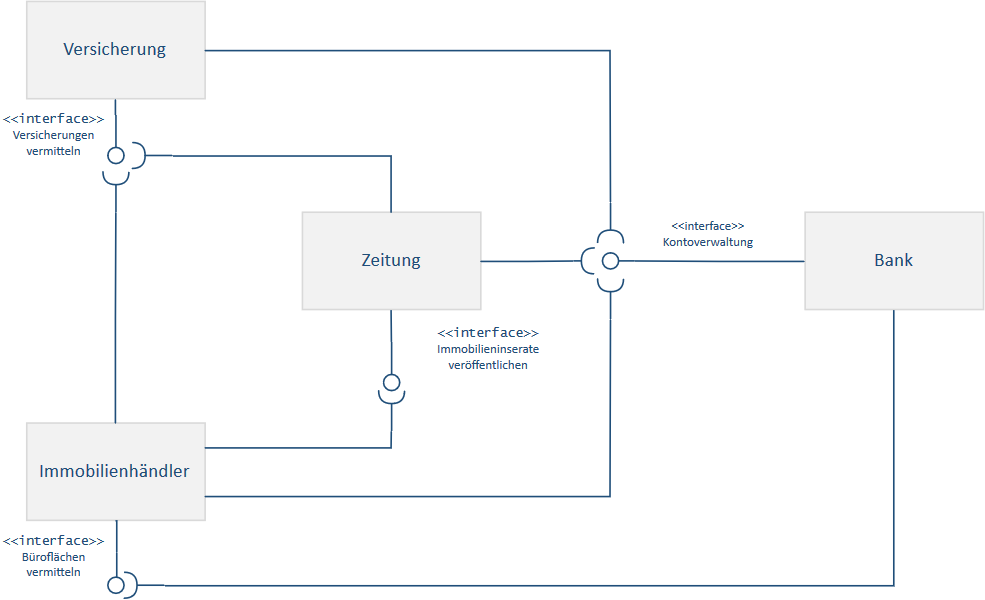
\includegraphics[scale=0.6]{pics/diagrams/gesamtsystem.png}
\caption{Übersicht über das Gesamtsystem}
\label{fig:gesamtsystem}
\end{figure}

\section{Immobilieninserate}
Sharkz soll seinen Benutzern ermöglichen, Anzeigen für Objekte aus der Immobilienbranche online zu veröffentlichen.

\subsection{Attribute}
Der Kunde soll die Möglichkeit haben, gewisse Angaben zum dem Objekt, welches er mit bewirbt, zu machen. Zwingende Attribute sind die \textit{Angebotsart} (Vermieten/Verkaufen) und die \textit{Art der Immobilie} (Haus/Wohnung/Büro) sowie \textit{Grundstücks- und Wohnfläche} und die \textit{Anzahl der Zimmer}. Außerdem verpflichtend ist die Angabe des \textit{Preises}. Des Weiteren sollen optional \textit{Bilder} hinzugefügt werden können und ein \textit{Beschreibungstext} angezeigt werden.
\newline
Damit der Kunde von Interessenten kontaktiert werden kann, muss eine \textit{Telefonnummer oder eine E-Mail-Adresse} angezeigt werden.
\newline
Für die Abrechnung muss der Kunde auch entweder einen \textit{Zeitraum} angeben, in dem sein Inserat öffentlich sichtbar ist, oder ein spezifisches Einstelldatum.

\chapter{Design}

\chapter{Implementierung}

\chapter{Test}

\chapter{Fazit}

\end{document}